Lattice gauge theory formulates QCD on a discrete Euclidean spacetime lattice, thereby transforming the
infinite-dimensional quantum field theory path integral into a finite-dimensional integral that can be solved
numerically with Monte Carlo methods and importance sampling.
In practice, lattice-QCD simulations are computationally intensive and require the use of the world's most
powerful computers.
The QCD Lagrangian has $1 + N_f + 1$ parameters: the gauge coupling $g^2$, the $N_f$ quark masses $m_f$, and 
the $CP$-violating parameter $\bar{\theta}$.
Because measurements of the neutron electric dipole moment (EDM) bound $\bar{\theta} < 10^{-10}$, most
lattice-QCD simulations set $\bar{\theta} = 0$.
The gauge-coupling and quark masses in lattice-QCD simulations are tuned by calibrating to $1 + N_f$
experimentally-measured quantities, typically hadron masses or mass-splittings.
Once the parameters of the QCD action are fixed, everything else is a prediction of QCD.

There are many ways to discretize QCD, particularly the fermions, but all of them recover QCD in the
continuum limit, i.e., when the lattice spacing $a\to 0$.
The various fermion formulations in use have different advantages (such as computational speed or exact
chiral symmetry) and different sources of systematic uncertainty; hence it is important to compute quantities
with more than one method for independent validation of results.
The time required for numerical simulations increases as the quark mass decreases (the condition number of
the Dirac operator, which must be inverted, increases with decreasing mass), so quark masses in lattice
simulations have usually been higher than those in the real world.
Typical lattice calculations now use quark masses such that the pion mass $m_\pi \lesssim 300$~MeV, while 
state-of-the art calculations for some quantities attain pions at or slightly below the physical mass of 
$m_\pi\sim140$~MeV. 
Over the coming decade, improvements in algorithms and increases in computing power will render chiral
extrapolations unnecessary.

Most lattice-QCD simulations proceed in two steps.
First one generates an ensemble of gauge fields with a distribution $\exp[-S_\text{QCD}]$; next one
computes operator expectation values on these gauge fields.
A major breakthrough in lattice-QCD occurred with the advent of gauge-field ensembles that include the
effects of the dynamical $u$, $d$, and $s$ quarks in the vacuum.
Lattice-QCD simulations now regularly employ ``$N_f = 2+1$" sea quarks in which the light $u$ and $d$
sea-quark masses are degenerate and somewhat heavier than the physical values, and the strange-sea quark mass
takes its physical value.
Further, ``$N_f = 2 + 1 + 1$" simulations that include a charm sea quark are now underway; dynamical charm
effects are expected to become important as precision for some quantities reaches the percent level.
During the coming decade, even $N_f=1+1+1+1$ simulations which include isospin-breaking in the sea are
planned.

The easiest quantities to compute with controlled systematic errors and high precision in lattice-QCD
simulations have only a hadron in the initial state and at most one hadron in the final state, where the
hadrons are stable under QCD (or narrow and far from threshold).
These quantities, often referred to as ``gold-plated,'' include meson masses and decay constants,
semileptonic and rare decay form factors, and neutral meson mixing parameters, and enable determinations of
all CKM matrix elements except $|V_{tb}|$.
Many interesting QCD observables are not gold-plated, however, such as resonances like the $\rho$ and $K^*$
mesons, fully hadronic decay matrix elements such as for $K \to \pi\pi$ and $B\to DK$, and long-distance
dominated quantities such as $D^0$-$\bar{D}^0$~mixing.
That said, lattice QCD with current resources is beginning to tackle such quantities, particularly in 
$K\to\pi\pi$ decay.

Many errors in lattice-QCD calculations can be assessed within the framework of effective field theory.
Lattice-QCD calculations typically quote the following sources of uncertainty:
%
\begin{itemize}
\item \emph{Monte Carlo statistics and fitting};
\item \emph{tuning lattice spacing and quark masses} by calibrating to a few experimentally-measured 
quantities such as $m_\pi$, $m_K$, $m_{D_s}$, $m_{B_s}$, $m_\Omega$, and $f_\pi$;
\item \emph{matching lattice gauge theory to continuum QCD} using fixed-order lattice perturbation theory, 
step-scaling, or other partly or fully nonperturbative methods;
\item \emph{chiral and continuum extrapolation} by simulating at a sequence of light (up and down) quark
masses and lattice spacings and extrapolating to $m_{\rm lat} \to m_{\rm phys}$ and $a\to0$ using functional
forms derived in chiral and weak-coupling QCD perturbation theory;
\item \emph{finite volume corrections}, which may be estimated using effective theory and/or studied directly 
by simulating lattices with different spatial volumes.
\end{itemize}
%
The methods for estimating uncertainties can be verified by comparing results for known quantities with
experiment.
Lattice-QCD calculations successfully reproduce the experimentally-measured low-lying hadron
spectrum~\cite{Aubin:2004wf,Aoki:2008sm,Durr:2008zz,Bazavov:2009bb,Christ:2010dd,Bernard:2010fr,Gregory:2010gm,Dudek:2011tt,Bietenholz:2011qq,Mohler:2011ke,Gregory:2011sg}, as shown in Fig.~\ref{lqcd:fig:spectrum}.
Lattice-QCD results agree with nonlattice determinations of the charm-and bottom-quark
masses~\cite{Chetyrkin:2009fv,McNeile:2010ji,Beringer:1900zz} and strong coupling~$\alpha_s$
\cite{McNeile:2010ji,Allison:2008xk,Davies:2008sw,Aoki:2009tf,Shintani:2010ph,Bethke:2011tr,Blossier:2012ef}, but now surpass the precision obtained by other methods.
Further, lattice-QCD calculations correctly predicted the mass of the $B_c$
meson~\cite{Allison:2004be,Abulencia:2005usa}, the leptonic decay constants $f_D$ and
$f_{D_s}$~\cite{Aubin:2005ar,Artuso:2005ym}, and the $D\to K \ell \nu$ semileptonic form
factor~\cite{Aubin:2004ej,Widhalm:2006wz} (see Fig.~\ref{lqcd:fig:D2K}) before the availability of precise
experimental measurements.
These successful predictions and postdictions validate the methods of numerical lattice QCD, and demonstrate
that reliable results can be obtained with controlled uncertainties.

\begin{figure}
    \centering
    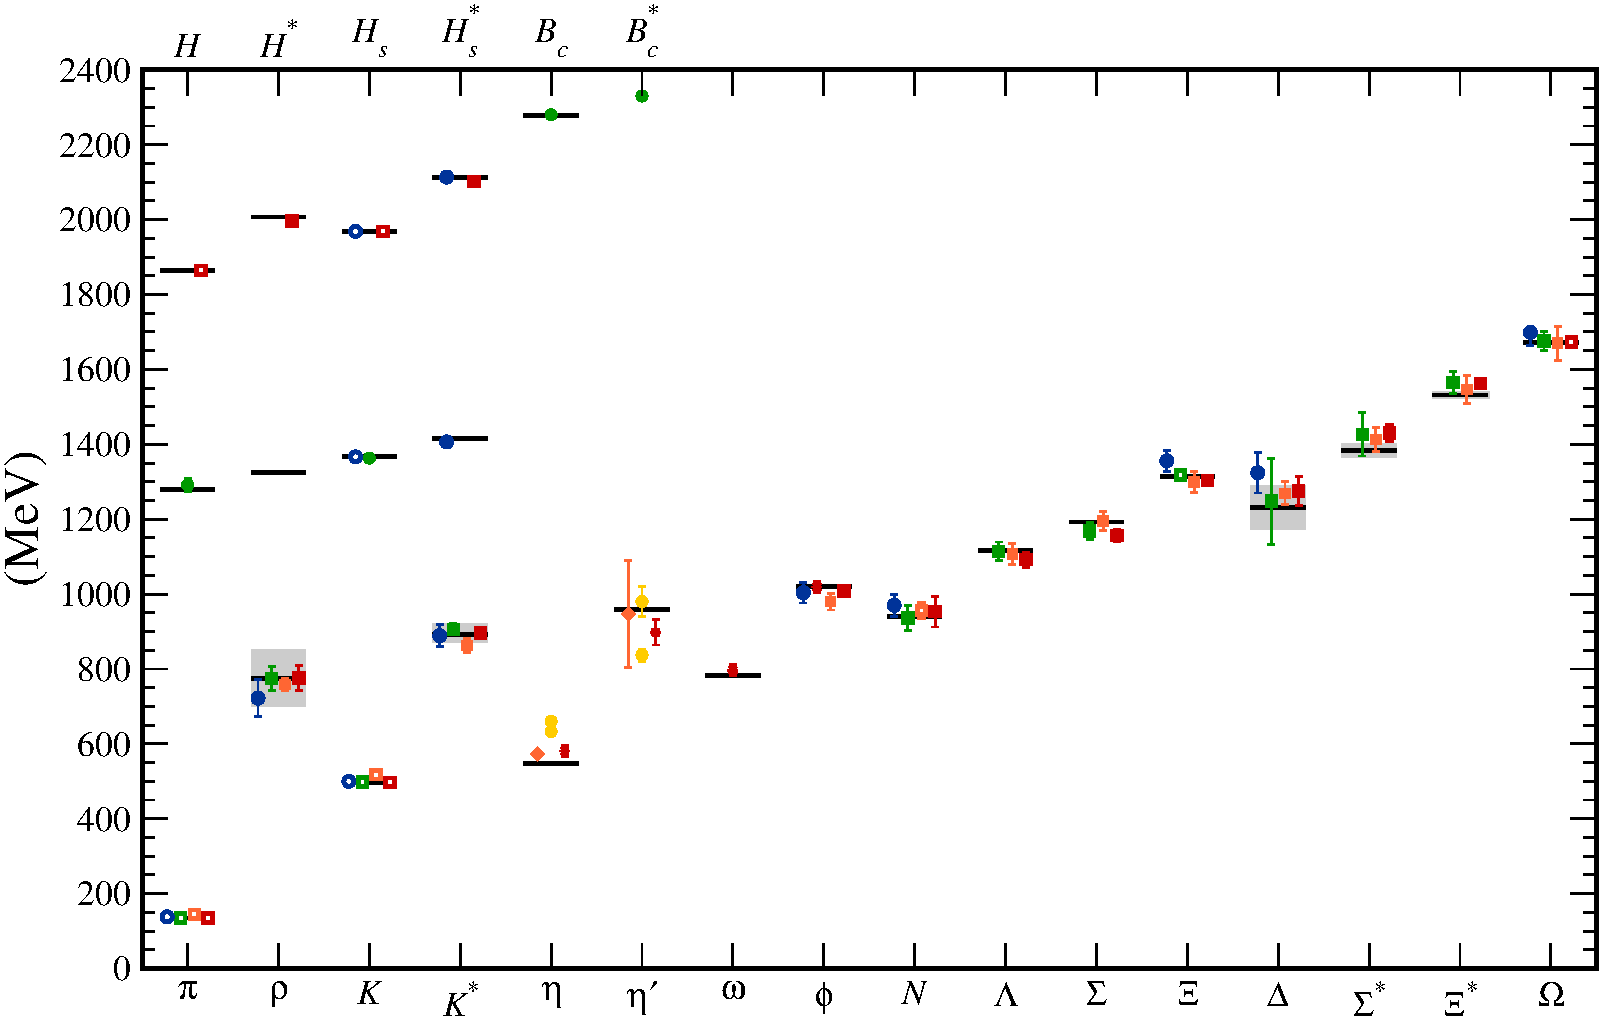
\includegraphics[width=\linewidth]{CpF-T3/spectrum.pdf}
    \caption[Hadron spectrum from many different lattice-QCD calculations]{Hadron spectrum from many 
        different lattice-QCD calculations~\cite{Aubin:2004wf,Aoki:2008sm,Durr:2008zz,Bazavov:2009bb,Christ:2010dd,Bernard:2010fr,Gregory:2010gm,Dudek:2011tt,Bietenholz:2011qq,Mohler:2011ke,Gregory:2011sg}.
        Open symbols denote masses used to fix bare parameters; closed symbols represent \emph{ab initio}
        calculations.
        Horizontal black bars (gray boxes) show the experimentally measured masses (widths).
        $b$-flavored meson masses ($B_c^{(*)}$ and $H_{(s)}^{(*)}$ near 1300~MeV) are offset by $-4000$~MeV.
        Circles, squares and diamonds denote staggered, Wilson and domain-wall fermions, respectively.
        Asterisks represent anisotropic lattices ($a_t/a_s<1$).
        Red, orange, yellow and green and blue signify increasing ensemble sizes (i.e., increasing range of 
        lattice spacings and quark masses).
        From Ref.~\cite{Kronfeld:2012uk}.}
    \label{lqcd:fig:spectrum}
\end{figure}

\begin{figure}
    \centering
    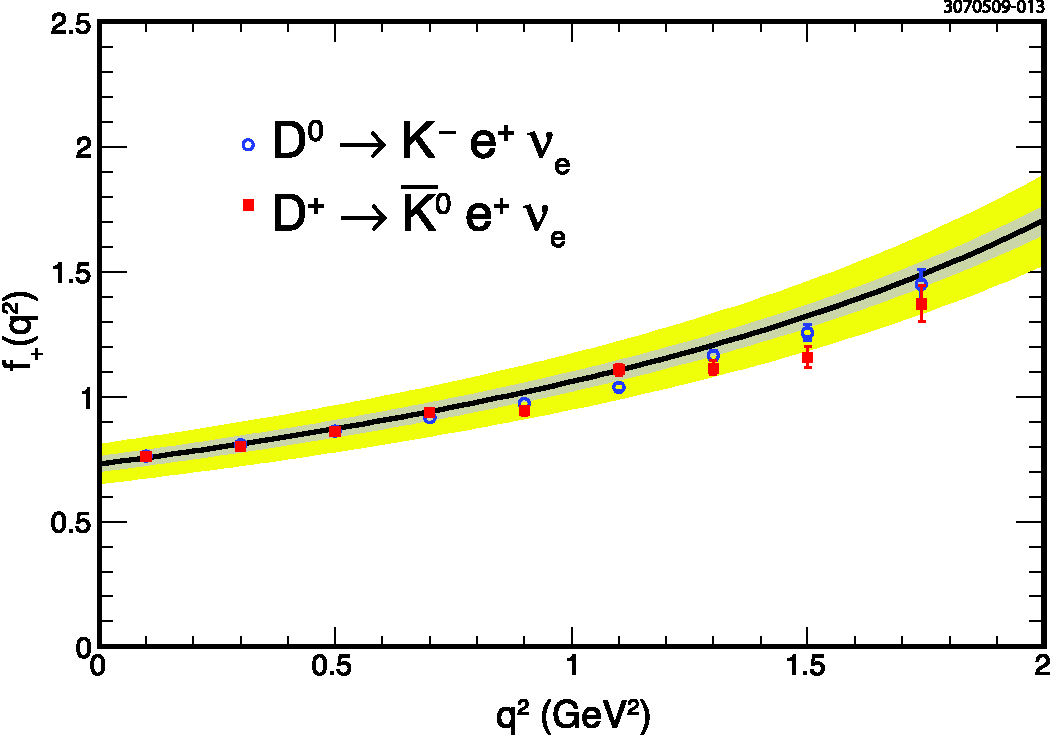
\includegraphics[width=0.495\textwidth]{CpF-T3/D2K.pdf}\hfill
    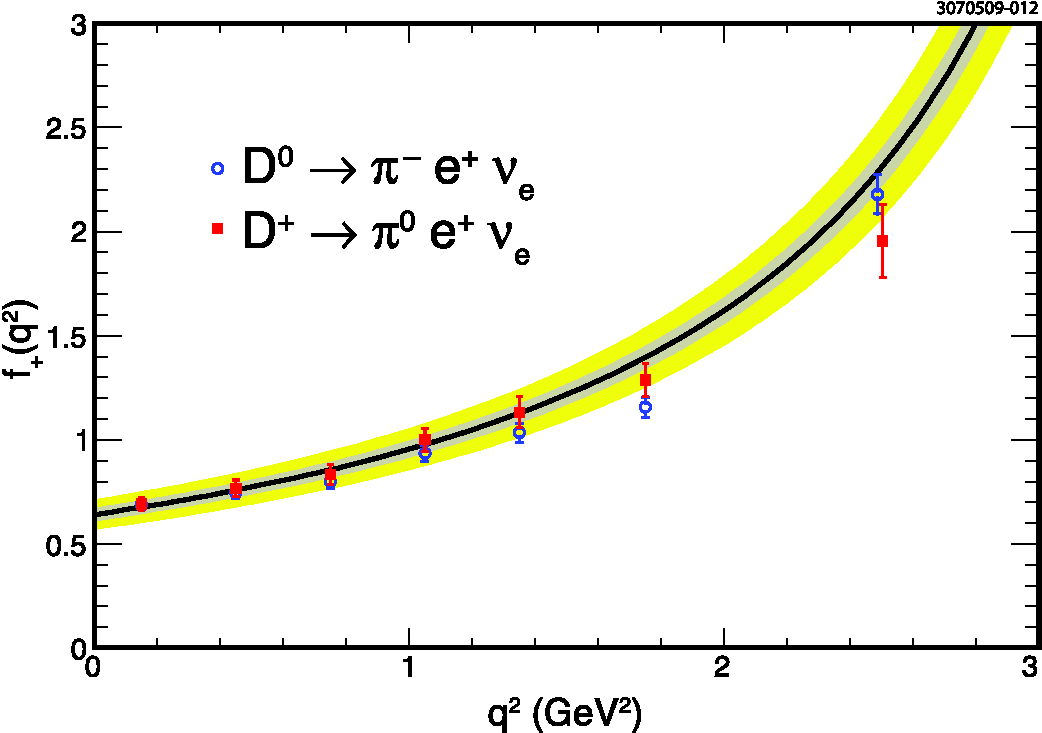
\includegraphics[width=0.495\textwidth]{CpF-T3/D2pi.pdf}
    \caption[Lattice-QCD calculations of $D$-meson form factors compared with measurements]{Comparison of 
        $N_f = 2+1$ lattice-QCD calculations of $D$-meson form factors~\cite{Aubin:2004ej,Bernard:2009ke} 
        (curves with error bands) with measurements from CLEO~\cite{Besson:2009uv} (points with error bars).
        From Ref.~\cite{Besson:2009uv}.}
    \label{lqcd:fig:D2K}
\end{figure}

In the last five years lattice QCD has matured into a precision tool.
Results with fully controlled errors are available
for nearly twenty matrix elements:
the decay constants
$f_\pi$, $f_K$, $f_D$, $f_{D_s}$, $f_B$ and $f_{B_s}$, 
semileptonic form factors for
$K\to \pi$, $D \to K$, $D\to\pi$, 
$B\to D$, $B\to D^{*}$, $B_s\to D_s$ and $B\to\pi$,
and the four-fermion mixing matrix elements
$B_K$, $f_B^2 B_B$ and $f_{B_s}^2 B_{B_s}$.
By contrast, in 2007, 
only $f_K/f_\pi$ was fully controlled~\cite{whitepaper07}.
The present lattice errors for a sample of matrix elements relevant for the CKM unitarity-triangle fit, along with forecasts for the anticipated lattice errors in five years, can be found in the ``Report of the Quark Flavor Phyics" working group in these proceedings or in Ref.~\cite{USQCD_IF_whitepaper13}.
In the kaon sector, errors are at or below the percent level,
while for $D$ and $B$ mesons errors range from few to $\sim$10\%.  Because these matrix elements cannot be obtained directly from experiment,  it is important to cross-check these results with independent calculations using different lattice actions and analysis methods.  Indeed, this has been done for almost all the quantities noted above. 
This situation has spawned two lattice averaging efforts, 
{\tt latticeaverages.org}~\cite{Laiho:2009eu} and 
FLAG-1~\cite{Colangelo:2010et}, 
which have recently joined forces and expanded to form a worldwide
Flavor Lattice Averaging Group (FLAG-2), 
with first publication expected in mid-2013.

